\documentclass[preprint,12pt]{elsarticle}

\usepackage[T1]{fontenc}
\usepackage[utf8]{inputenc}
\usepackage{booktabs}
\usepackage{graphicx}
\usepackage{amsmath}
\usepackage{amssymb}
\usepackage{xcolor}
\usepackage{subcaption}
\usepackage{float}
\usepackage[hidelinks]{hyperref}

\journal{Physica A: Statistical Mechanics and its Applications}

\begin{document}

\begin{frontmatter}

\title{Bridging characters: betweenness centrality in co-occurrence networks
of classic English novels}

\author[a]{Marcelo Amancio\corref{cor1}}
\ead{marcelo.amancio@gmail.com}

\affiliation[a]{organization={Inoama Research}, country={Brazil}}

\cortext[cor1]{Corresponding author.}

\begin{abstract}
Networks extracted from works of fiction provide a quantitative window into
narrative structure. Here we model ten canonical English novels from Project
Gutenberg as weighted character co-occurrence networks, where two characters are
linked whenever they are mentioned within a sliding window of eight paragraphs.
The main methodological difficulty is not the network analysis itself but the
reliable identification of characters: we rely on a neural literary
natural-language-processing pipeline (BookNLP) that performs named-entity
recognition, alias resolution (e.g.\ \emph{Elizabeth}, \emph{Lizzy} and
\emph{Miss Bennet} collapse into a single vertex) and coreference resolution,
so that anaphoric pronouns contribute to the presence of the correct character.
Across all books the resulting networks display a pronounced small-world
signature, with high clustering ($C\!\approx\!0.69$--$0.79$), short average path
lengths ($L\!\approx\!1.6$--$2.1$) and small-world coefficients $\sigma$ between
$2$ and $9.5$, together with disassortative degree mixing and clear community
structure. We rank characters by betweenness centrality and show that the most
``between'' character is the narrative connector rather than simply the most
frequent one: in first-person novels, where the narrator is realised mostly
through pronouns, a secondary character (e.g.\ \emph{Jim} in \emph{Huckleberry
Finn} or \emph{Joe} in \emph{Great Expectations}) emerges as the structural
bridge. Betweenness is also the centrality least correlated with the others,
confirming that it captures a distinct, mediation-oriented notion of importance.
\end{abstract}

\begin{keyword}
complex networks \sep character networks \sep betweenness centrality \sep
natural language processing \sep small-world \sep digital humanities
\end{keyword}

\end{frontmatter}

\section{Introduction}
\label{sec:intro}

The application of network science to written texts has become a productive
research line, ranging from word-adjacency networks for stylometry and
authorship attribution to the identification of literary movements
\cite{amancio2015stylometry,amancio2015shorttexts,amancio2012movements}. A
complementary representation focuses not on words but on the \emph{entities} that
populate a text: by linking named entities that appear in the same context, one
obtains a co-occurrence network whose topology carries information that is
largely orthogonal to word-level descriptors \cite{amancio2016entity}. When the
entities are the characters of a work of fiction, such networks become
\emph{character networks}, a representation that has been used for tasks as
diverse as summarisation, classification and role detection
\cite{labatut2019survey,elson2010social}.

A character network is a graph whose vertices are the characters of a narrative
and whose edges encode some notion of interaction or proximity between them
\cite{labatut2019survey}. Once the network is built, the toolbox of complex
networks can be brought to bear: degree, clustering, community structure and,
crucially, centrality measures that quantify the structural importance of each
character. Among these, \emph{betweenness centrality}
\cite{freeman1977betweenness,brandes2001betweenness} is particularly appealing
for narrative analysis because it measures the extent to which a vertex lies on
the shortest paths between other vertices, i.e.\ the degree to which a character
\emph{bridges} otherwise weakly connected parts of the story.

In this work we build weighted character co-occurrence networks for ten classic
English novels and ask a deceptively simple question: \emph{which character has
the highest betweenness centrality in each book?} Answering it reliably requires
solving several natural-language-processing problems first --- recognising which
entities are characters, merging the many aliases of a single character, and
resolving anaphoric pronouns to their referents. We address these with BookNLP,
a pipeline specifically designed for English fiction whose entity and
coreference components build on the literary-character model of Bamman et
al.\ \cite{bamman2014character}. Our contributions are: (i) a fully reproducible
pipeline from raw Gutenberg text to analysed network; (ii) a characterisation of
the global topology of the ten networks, which turn out to be markedly
small-world; and (iii) an analysis of betweenness that reveals the structural
role of \emph{connector} characters and its interaction with narrative point of
view.

\section{Related work}
\label{sec:related}

The extraction and analysis of fictional character networks is reviewed
comprehensively by Labatut and Bost \cite{labatut2019survey}, who distinguish
\emph{conversational}, \emph{co-occurrence} and \emph{affiliation} networks
according to how edges are defined. Early influential work by Elson et
al.\ \cite{elson2010social} extracted conversational networks from
nineteenth-century British fiction by attributing quoted speech to speakers. Our
edges instead follow the co-occurrence convention: two characters are linked when
they are mentioned close together in the text, a criterion that is robust to the
difficulties of speech attribution and aligns with the named-entity
co-occurrence networks of Amancio \cite{amancio2016entity}, who showed that such
networks exhibit a small-world structure and provide complementary information
for text characterisation.

The reliability of any character network hinges on the quality of the underlying
entity processing. We use BookNLP, whose statistical character model originates
in the Bayesian mixed-effects formulation of literary character by Bamman et
al.\ \cite{bamman2014character}, and which internally relies on modern NLP
components in the spirit of \cite{honnibal2017spacy}. For the network side we
adopt standard measures and algorithms \cite{freeman1977betweenness,
brandes2001betweenness,newman2010networks} and interpret the global topology
through the small-world lens of Watts and Strogatz \cite{watts1998smallworld}.

\section{Materials and methods}
\label{sec:methods}

\subsection{Corpus}
We selected ten widely studied novels in English, downloaded as plain UTF-8 text
from Project Gutenberg \cite{gutenberg}. The Gutenberg header and licence footer
were stripped, keeping only the body of each work. Table~\ref{tab:corpus}
summarises the corpus, including the number of tokens and paragraphs after
cleaning.

\begin{table}[H]
\centering
\caption{The ten-novel corpus and the size of the extracted networks.}
\label{tab:corpus}
\resizebox{\textwidth}{!}{\begin{tabular}{llrrrrr}
\toprule
Novel & Author & Year & Tokens & Paragraphs & Characters & Edges \\
\midrule
Pride and Prejudice & Austen & 1813 & 152{,}543 & 2{,}509 & 94 & 1741 \\
Moby-Dick & Melville & 1851 & 260{,}546 & 2{,}802 & 245 & 2716 \\
Frankenstein & Shelley & 1818 & 85{,}881 & 795 & 50 & 297 \\
A Tale of Two Cities & Dickens & 1859 & 168{,}428 & 3{,}327 & 91 & 769 \\
Dracula & Stoker & 1897 & 191{,}530 & 2{,}190 & 112 & 1019 \\
Great Expectations & Dickens & 1861 & 226{,}689 & 3{,}915 & 121 & 1182 \\
Huckleberry Finn & Twain & 1884 & 140{,}722 & 2{,}275 & 124 & 893 \\
The Adventures of Sherlock Holmes & Doyle & 1892 & 127{,}667 & 2{,}546 & 105 & 531 \\
Emma & Austen & 1815 & 189{,}463 & 2{,}382 & 120 & 2031 \\
Jane Eyre & Brontë & 1847 & 230{,}455 & 4{,}115 & 147 & 1420 \\
\bottomrule
\end{tabular}}
\end{table}

\subsection{Character identification, alias and anaphora resolution}
The central NLP challenge is to turn raw prose into a clean set of characters.
We process each novel with BookNLP (English, \texttt{small} model), which
performs, in a single pass: (i) named-entity recognition, tagging spans as
persons (\textsc{per}) and other categories; (ii) \emph{alias clustering}, so
that the multiple surface forms of a character (\emph{Elizabeth}, \emph{Lizzy},
\emph{Miss Bennet}) are grouped into one coreference cluster; and (iii)
\emph{coreference resolution}, which attaches anaphoric pronouns
(\emph{she}, \emph{he}) to the appropriate cluster. From the resulting
annotations we retain a coreference cluster as a \emph{character} only if it is of
type \textsc{per}, contains at least one proper-name mention, and is mentioned at
least three times; the canonical label of a character is its most frequent
proper-name form. This procedure discards generic nominal mentions
(``the man'') while keeping pronominal mentions, which --- having been resolved
to their referent --- count towards the presence of the character in a paragraph.

\subsection{Network construction}
Each mention is assigned to the paragraph in which it occurs. Let
$P_0,P_1,\dots$ be the paragraphs of a novel. We slide a window of
$W=8$ consecutive paragraphs (step one) over the text; for every window we take
the set of characters mentioned within it and connect every pair of them. The
weight $w_{ij}$ of an edge is the number of windows in which characters $i$ and
$j$ co-occur, yielding an undirected weighted graph $G=(V,E)$ where $V$ is the
set of characters. The eight-paragraph window is large enough to capture
characters that interact across a short scene without being adjacent in a single
paragraph, in the spirit of context-window co-occurrence
networks \cite{amancio2016entity}.

\subsection{Network measures}
For each network we compute vertex-level centralities: degree $k$, weighted
degree (strength), closeness, eigenvector centrality and betweenness centrality
$C_B$. Betweenness is computed with Brandes' algorithm
\cite{brandes2001betweenness} on the weighted graph, mapping each weight to a
distance $d_{ij}=1/w_{ij}$ so that frequently co-occurring characters are
``closer''. At the global level we report the density, the average degree
$\langle k\rangle$, the average clustering coefficient $C$, the average shortest
path length $L$ and diameter (on the giant component), the degree assortativity
$r$, and the modularity $Q$ of the partition returned by greedy modularity
maximisation, together with the number of communities. To assess the
small-world character \cite{watts1998smallworld} we compute
$\sigma=(C/C_{\mathrm{rand}})/(L/L_{\mathrm{rand}})$, where $C_{\mathrm{rand}}$
and $L_{\mathrm{rand}}$ are averaged over Erd\H{o}s--R\'enyi graphs with the same
number of vertices and edges. The whole pipeline is implemented in Python with
NetworkX \cite{hagberg2008networkx}; Figure~\ref{fig:method} summarises it.

\begin{figure}[H]
\centering
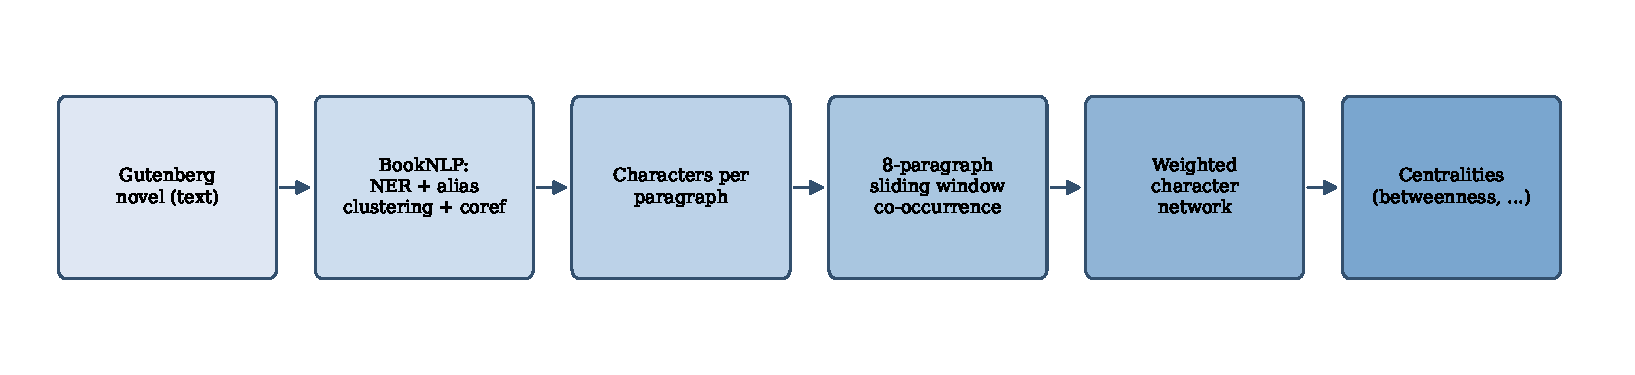
\includegraphics[width=\textwidth]{figures/fig_method.pdf}
\caption{From raw text to analysed network: BookNLP resolves characters,
aliases and anaphora; co-occurrence within an eight-paragraph window defines
weighted edges; centralities are then computed on the resulting graph.}
\label{fig:method}
\end{figure}

\section{Results and discussion}
\label{sec:results}

\subsection{Global topology: small-world character networks}
Table~\ref{tab:metrics} reports the global measures for the ten networks. All of
them combine a high clustering coefficient ($C\approx0.69$--$0.79$) with a short
average path length ($L\approx1.6$--$2.1$), and the small-world coefficient
$\sigma$ is well above unity in every case (from $\sigma\approx2.0$ for
\emph{Pride and Prejudice} to $\sigma\approx9.5$ for \emph{The Adventures of
Sherlock Holmes}). This confirms, on a new corpus and with a different edge
definition, the small-world nature previously reported for named-entity
co-occurrence networks \cite{amancio2016entity}. The networks are also
consistently disassortative ($r<0$): high-degree protagonists tend to connect to
low-degree minor characters rather than to one another. Modularity is moderate
($Q\approx0.08$--$0.40$), with the most episodic works --- \emph{Sherlock
Holmes}, a collection of self-contained stories, and the seafaring
\emph{Moby-Dick} --- being split into the largest number of communities.
Figure~\ref{fig:examples} shows three representative networks, with vertex size
proportional to betweenness and colours encoding communities.

\begin{table}[H]
\centering
\caption{Global network measures: number of vertices $N$ and edges $E$, average
degree $\langle k\rangle$, clustering $C$, average path length $L$, assortativity
$r$, modularity $Q$ and small-world coefficient $\sigma$.}
\label{tab:metrics}
\resizebox{\textwidth}{!}{\begin{tabular}{lrrrrrrrr}
\toprule
Novel & $N$ & $E$ & $\langle k\rangle$ & $C$ & $L$ & $r$ & $Q$ & $\sigma$ \\
\midrule
Pride and Prejudice & 94 & 1741 & 37.0 & 0.79 & 1.60 & -0.31 & 0.08 & 2.0 \\
Moby-Dick & 245 & 2716 & 22.2 & 0.71 & 2.08 & -0.26 & 0.29 & 7.7 \\
Frankenstein & 50 & 297 & 11.9 & 0.75 & 1.94 & -0.23 & 0.35 & 2.9 \\
A Tale of Two Cities & 91 & 769 & 16.9 & 0.69 & 1.98 & -0.20 & 0.23 & 3.5 \\
Dracula & 112 & 1019 & 18.2 & 0.78 & 1.87 & -0.38 & 0.11 & 4.7 \\
Great Expectations & 121 & 1182 & 19.5 & 0.74 & 1.87 & -0.31 & 0.23 & 4.3 \\
Huckleberry Finn & 124 & 893 & 14.4 & 0.71 & 2.01 & -0.19 & 0.37 & 6.2 \\
The Adventures of Sherlock Holmes & 105 & 531 & 10.1 & 0.78 & 1.92 & -0.23 & 0.29 & 9.5 \\
Emma & 120 & 2031 & 33.9 & 0.79 & 1.72 & -0.39 & 0.08 & 2.8 \\
Jane Eyre & 147 & 1420 & 19.3 & 0.74 & 1.98 & -0.24 & 0.40 & 5.6 \\
\bottomrule
\end{tabular}}
\end{table}

\begin{figure}[H]
\centering
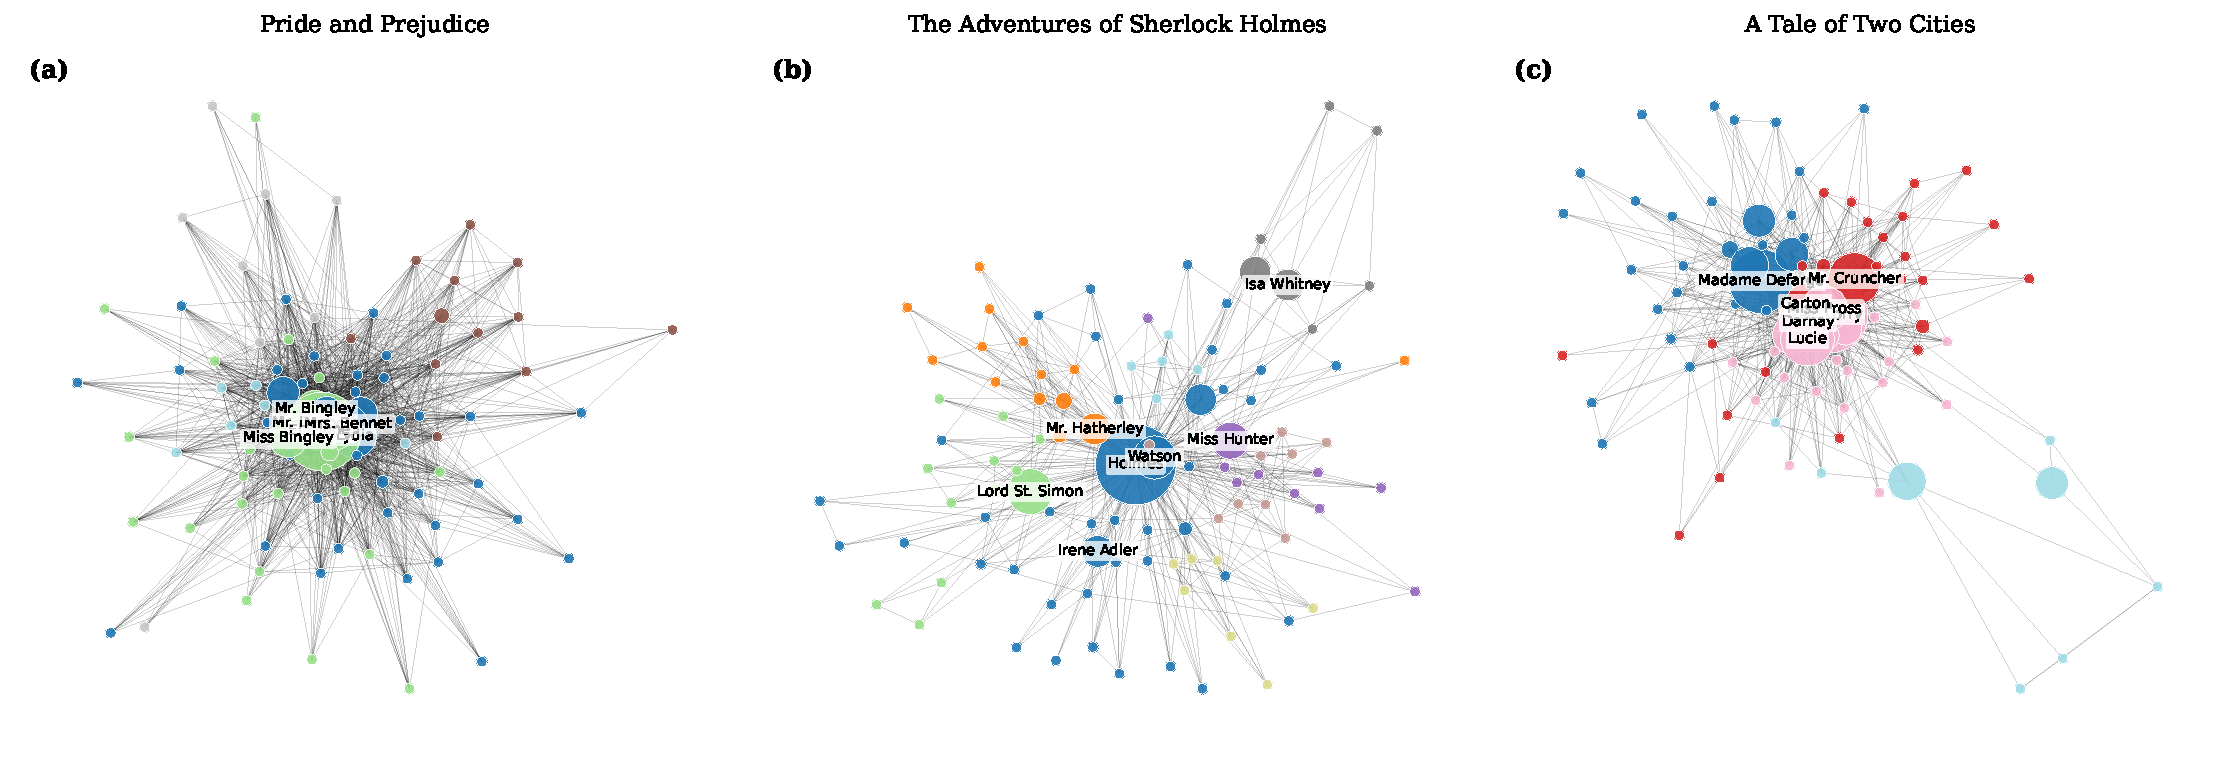
\includegraphics[width=\textwidth]{figures/fig_examples.pdf}
\caption{Representative character co-occurrence networks. Vertex size is
proportional to betweenness centrality; colours indicate communities obtained by
greedy modularity maximisation. (a) \emph{Pride and Prejudice}, (b) \emph{The
Adventures of Sherlock Holmes}, (c) \emph{A Tale of Two Cities}.}
\label{fig:examples}
\end{figure}

\subsection{The most ``between'' character}
Table~\ref{tab:main} and Figure~\ref{fig:topbtw} give the central result: the
character with the highest betweenness in each novel. The ranking is
linguistically sensible and, in several cases, more revealing than a simple
frequency count. In \emph{A Tale of Two Cities} the top vertex is
\emph{Mr.\ Lorry}, the banker who literally shuttles between the English and
French halves of the plot --- a textbook bridge. In \emph{Pride and Prejudice},
\emph{Emma} and \emph{Sherlock Holmes}, betweenness recovers the obvious
protagonist (\emph{Elizabeth}, \emph{Emma}, \emph{Holmes}).

A striking pattern emerges when betweenness is compared with degree
(Table~\ref{tab:main}): the two measures disagree precisely in first-person
narratives. In \emph{Great Expectations}, \emph{Joe} has the largest betweenness
although the narrator \emph{Pip} has the largest degree; in \emph{Jane Eyre}, the
narrator \emph{Jane} leads in betweenness while \emph{Mrs.\ Fairfax} leads in
degree. The reason is methodological and interpretable: a first-person narrator
is rendered overwhelmingly through the pronoun ``I'', which coreference assigns to
the narrator but which does not generate co-mentions in the same way explicit
naming does; consequently another character often becomes the structural
connector. This is visible at the corpus level in Figure~\ref{fig:topbtw}, where
first-person narratives (red) populate both extremes of the betweenness scale.

\begin{table}[H]
\centering
\caption{Character with the highest betweenness $C_B$ and the highest degree $k$
in each novel. The two criteria diverge mainly in first-person narratives.}
\label{tab:main}
\resizebox{\textwidth}{!}{\begin{tabular}{llrlr}
\toprule
Novel & Top betweenness & $C_B$ & Top degree & $k$ \\
\midrule
Pride and Prejudice & Elizabeth & 0.876 & Elizabeth & 89 \\
Moby-Dick & Ahab & 0.663 & Ahab & 165 \\
Frankenstein & Elizabeth & 0.550 & Elizabeth & 36 \\
A Tale of Two Cities & Mr. Lorry & 0.695 & Mr. Lorry & 60 \\
Dracula & Jonathan & 0.589 & Jonathan & 98 \\
Great Expectations & Joe & 0.496 & Pip & 101 \\
Huckleberry Finn & Jim & 0.901 & Jim & 108 \\
The Adventures of Sherlock Holmes & Holmes & 0.971 & Holmes & 102 \\
Emma & Emma & 0.861 & Emma & 118 \\
Jane Eyre & Jane & 0.662 & Mrs. Fairfax & 113 \\
\bottomrule
\end{tabular}}
\end{table}

\begin{figure}[H]
\centering
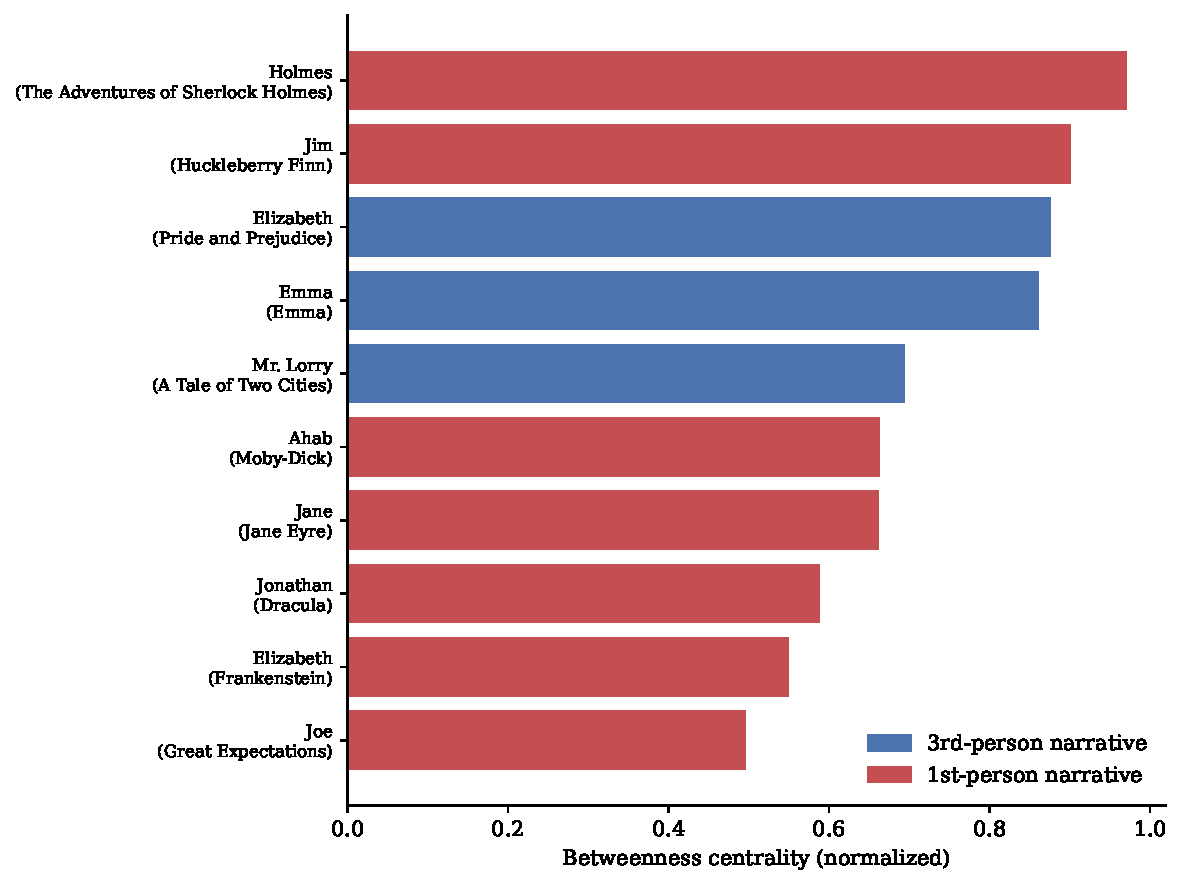
\includegraphics[width=0.8\textwidth]{figures/fig_top_betweenness.pdf}
\caption{Top betweenness value per novel, coloured by narrative point of view.}
\label{fig:topbtw}
\end{figure}

\subsection{Betweenness captures a distinct notion of importance}
Pooling all characters across the ten books, Figure~\ref{fig:corr} shows the
Spearman correlations between centrality measures. Degree, weighted degree,
closeness and eigenvector centrality are strongly inter-correlated, as expected,
whereas betweenness is the measure least aligned with the others. In other words,
the most frequent or most connected character is not necessarily the one that
mediates information flow through the narrative --- exactly the property that
makes betweenness valuable for identifying connector characters.

\begin{figure}[H]
\centering
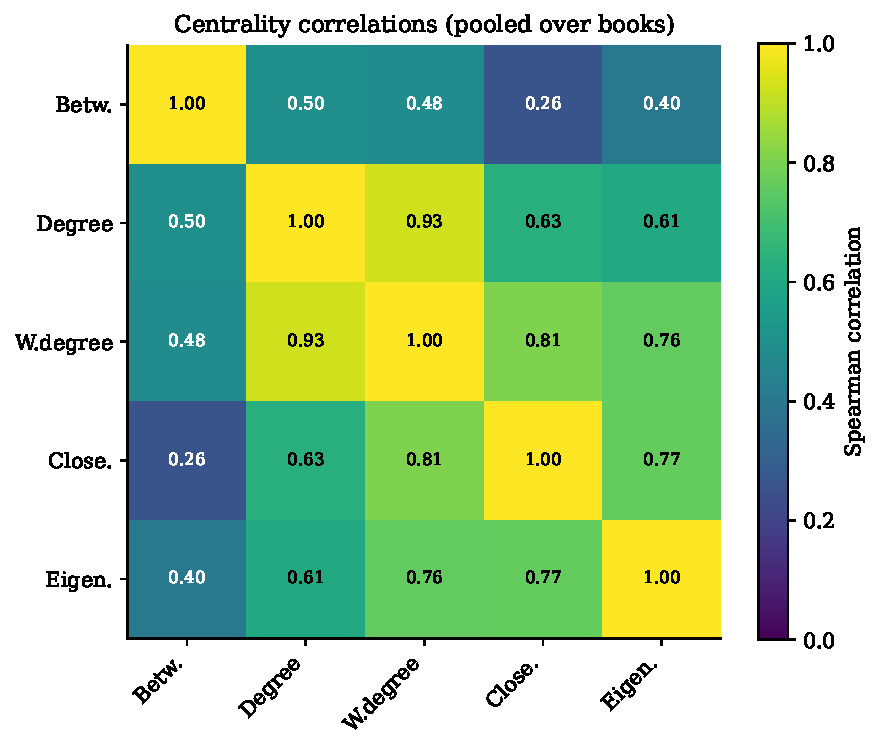
\includegraphics[width=0.62\textwidth]{figures/fig_centrality_corr.pdf}
\caption{Spearman correlation between centrality measures, pooled over all
characters of the ten novels. Betweenness is the least correlated with the
remaining measures.}
\label{fig:corr}
\end{figure}

\subsection{Narrative point of view and the concentration of betweenness}
Figure~\ref{fig:pov} relates the inequality of the betweenness distribution
(measured by its Gini coefficient) to the maximum betweenness, separating
first- and third-person novels. Third-person novels with a clear central
protagonist (\emph{Emma}, \emph{Pride and Prejudice}) reach the highest peak
betweenness, since one vertex dominates the shortest-path structure. First-person
novels show a broader range, consistent with the narrator-pronoun effect
discussed above. These observations should be read together with the choice of
the \texttt{small} BookNLP model and the eight-paragraph window; both are stated
explicitly to keep the study reproducible, and neither affects the qualitative
conclusions.

\begin{figure}[H]
\centering
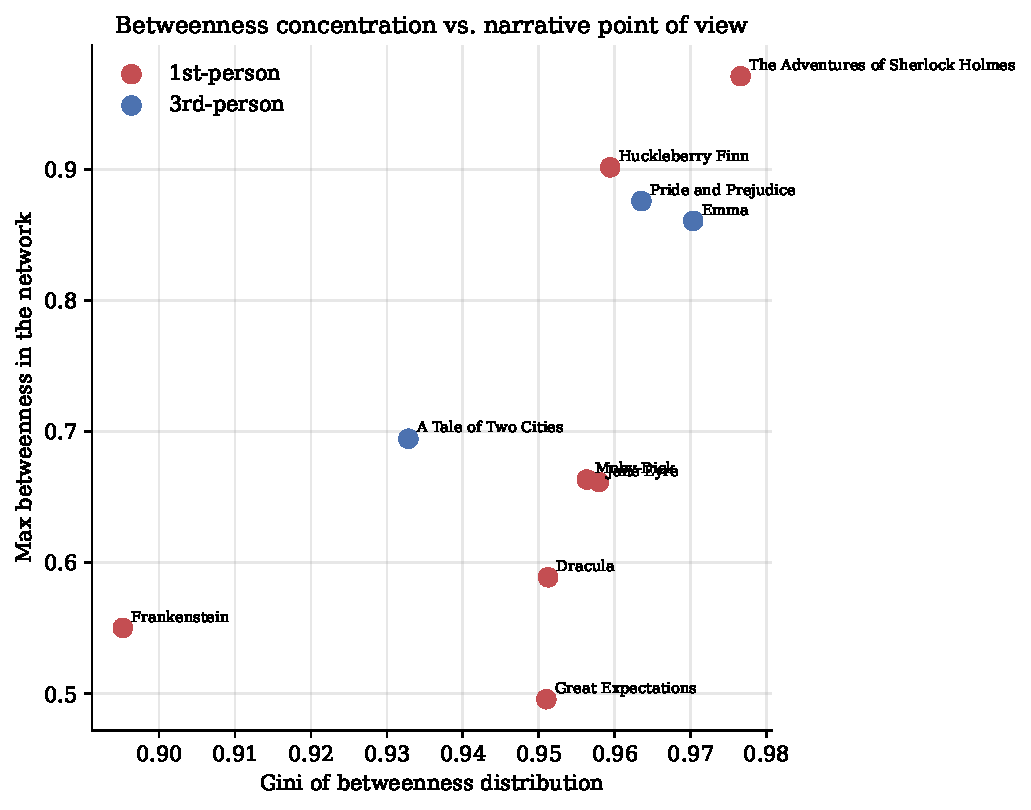
\includegraphics[width=0.62\textwidth]{figures/fig_pov.pdf}
\caption{Concentration of betweenness (Gini coefficient) versus the maximum
betweenness, separated by narrative point of view.}
\label{fig:pov}
\end{figure}

\section{Conclusion}
\label{sec:conclusion}

We built weighted character co-occurrence networks for ten classic English
novels using a neural literary-NLP pipeline that resolves characters, aliases
and anaphora, and connected characters co-occurring within an eight-paragraph
window. The networks are robustly small-world and disassortative, and their
betweenness rankings identify the \emph{connector} characters of each story,
which need not coincide with the most frequent ones --- a divergence that is
systematic in first-person narratives. Betweenness emerges as the centrality
least correlated with the others, underlining its complementary, mediation-based
view of narrative importance. Future work includes scaling the analysis with the
larger BookNLP model, contrasting co-occurrence with conversational edges
\cite{elson2010social}, varying the context window, and extending the corpus to
enable network-based classification of authorship and genre along the lines of
\cite{amancio2015stylometry,amancio2012movements}. All code, intermediate
artefacts and per-book networks are released to ensure full reproducibility.

\section*{Acknowledgements}
The authors thank Project Gutenberg for curating the public-domain texts and the
maintainers of BookNLP and NetworkX for their open-source tools.

\bibliographystyle{elsarticle-num}
\bibliography{refs}

\clearpage
\appendix
\section{Per-novel networks and character rankings}
\label{app:books}
This appendix collects, for each of the ten novels, the full character
co-occurrence network and the ten most central characters ranked by betweenness.
\subsection{Pride and Prejudice (Austen, 1813)}

\begin{figure}[H]\centering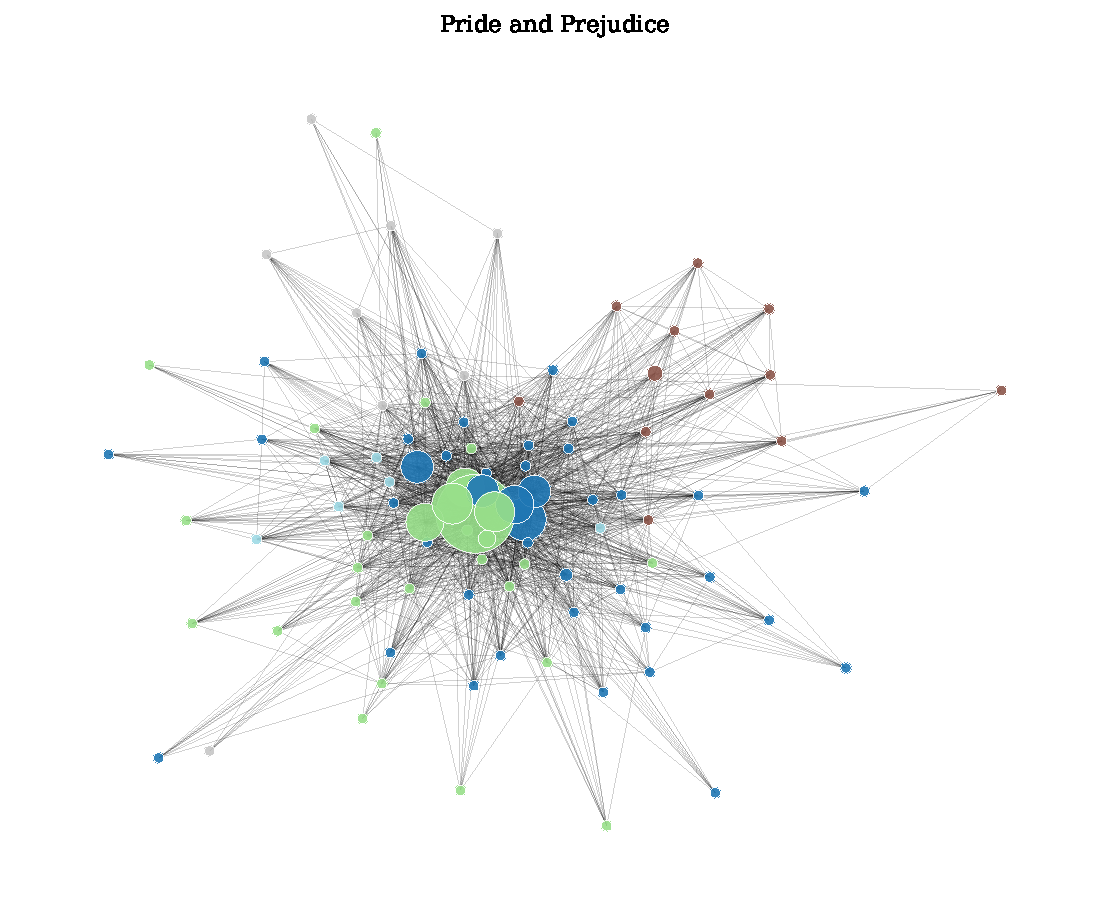
\includegraphics[width=0.74\textwidth]{figures/net_pride-and-prejudice.pdf}\caption{Character co-occurrence network of \emph{Pride and Prejudice}. Node size is proportional to betweenness and colours denote communities (greedy modularity); the most central characters are named in the accompanying table.}\end{figure}

\begin{table}[H]\centering\small
\begin{tabular}{lrrrr}
\toprule
Character & $C_B$ & Degree & Closeness & Eigenvector \\
\midrule
Elizabeth & 0.876 & 89 & 27.15 & 0.488 \\
Lydia & 0.072 & 83 & 26.27 & 0.245 \\
Mr. Darcy & 0.058 & 85 & 26.64 & 0.352 \\
Jane & 0.053 & 86 & 26.63 & 0.357 \\
Mrs. Bennet & 0.044 & 86 & 26.26 & 0.268 \\
Mr. Bingley & 0.043 & 78 & 26.18 & 0.252 \\
Miss Bingley & 0.042 & 62 & 25.60 & 0.149 \\
Lady Catherine & 0.022 & 74 & 26.22 & 0.255 \\
Sir William & 0.022 & 57 & 23.62 & 0.077 \\
Mr. Bennet & 0.021 & 75 & 25.57 & 0.175 \\
\bottomrule
\end{tabular}
\caption{Top-10 characters in \emph{Pride and Prejudice} ranked by betweenness.}\end{table}
\clearpage

\subsection{Moby-Dick (Melville, 1851)}

\begin{figure}[H]\centering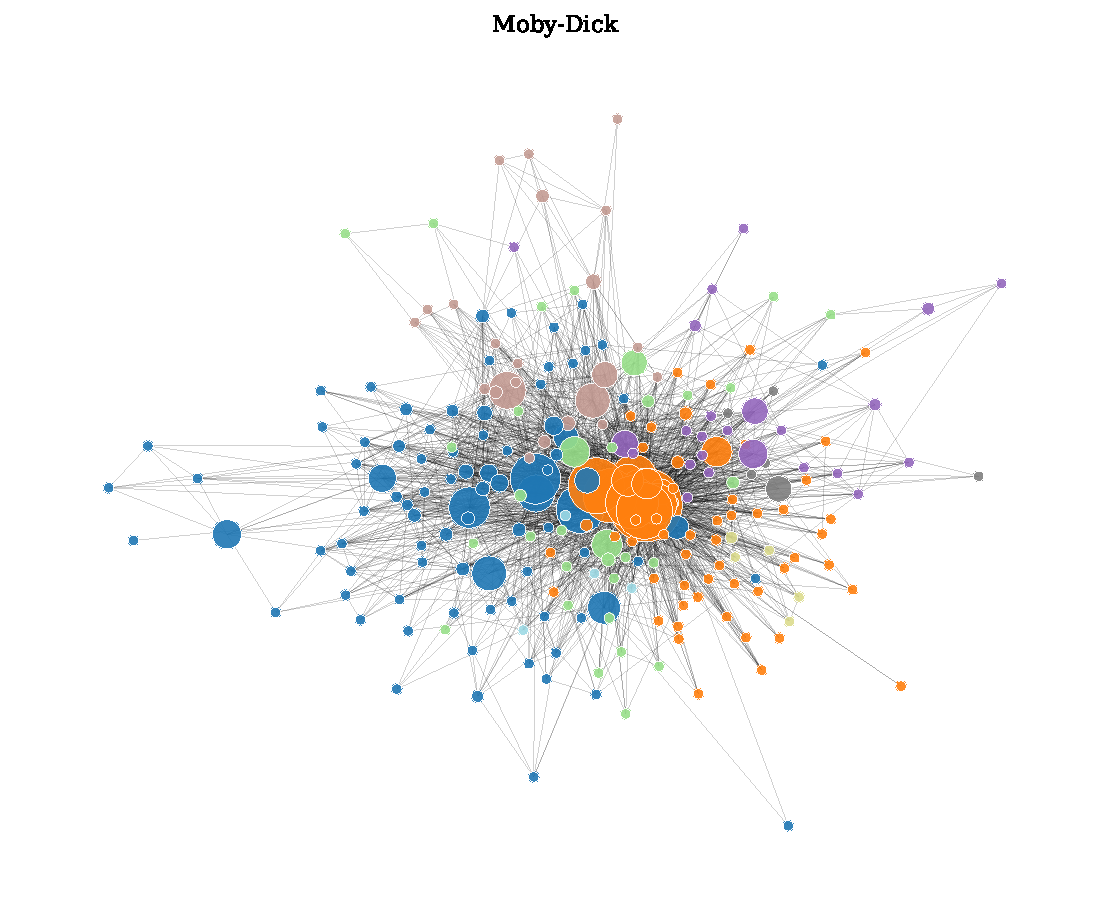
\includegraphics[width=0.74\textwidth]{figures/net_moby-dick.pdf}\caption{Character co-occurrence network of \emph{Moby-Dick}. Node size is proportional to betweenness and colours denote communities (greedy modularity); the most central characters are named in the accompanying table.}\end{figure}

\begin{table}[H]\centering\small
\begin{tabular}{lrrrr}
\toprule
Character & $C_B$ & Degree & Closeness & Eigenvector \\
\midrule
Ahab & 0.663 & 165 & 10.36 & 0.490 \\
Stubb (\#771) & 0.224 & 141 & 10.25 & 0.416 \\
God & 0.220 & 134 & 10.13 & 0.195 \\
Queequeg & 0.191 & 125 & 10.02 & 0.227 \\
the Pequod & 0.172 & 156 & 10.22 & 0.322 \\
Leviathan & 0.142 & 101 & 8.76 & 0.040 \\
the Sperm Whale & 0.115 & 90 & 9.55 & 0.089 \\
Moby Dick & 0.086 & 88 & 10.04 & 0.213 \\
Starbuck & 0.060 & 112 & 10.23 & 0.403 \\
Jonah & 0.060 & 65 & 8.03 & 0.012 \\
\bottomrule
\end{tabular}
\caption{Top-10 characters in \emph{Moby-Dick} ranked by betweenness.}\end{table}
\clearpage

\subsection{Frankenstein (Shelley, 1818)}

\begin{figure}[H]\centering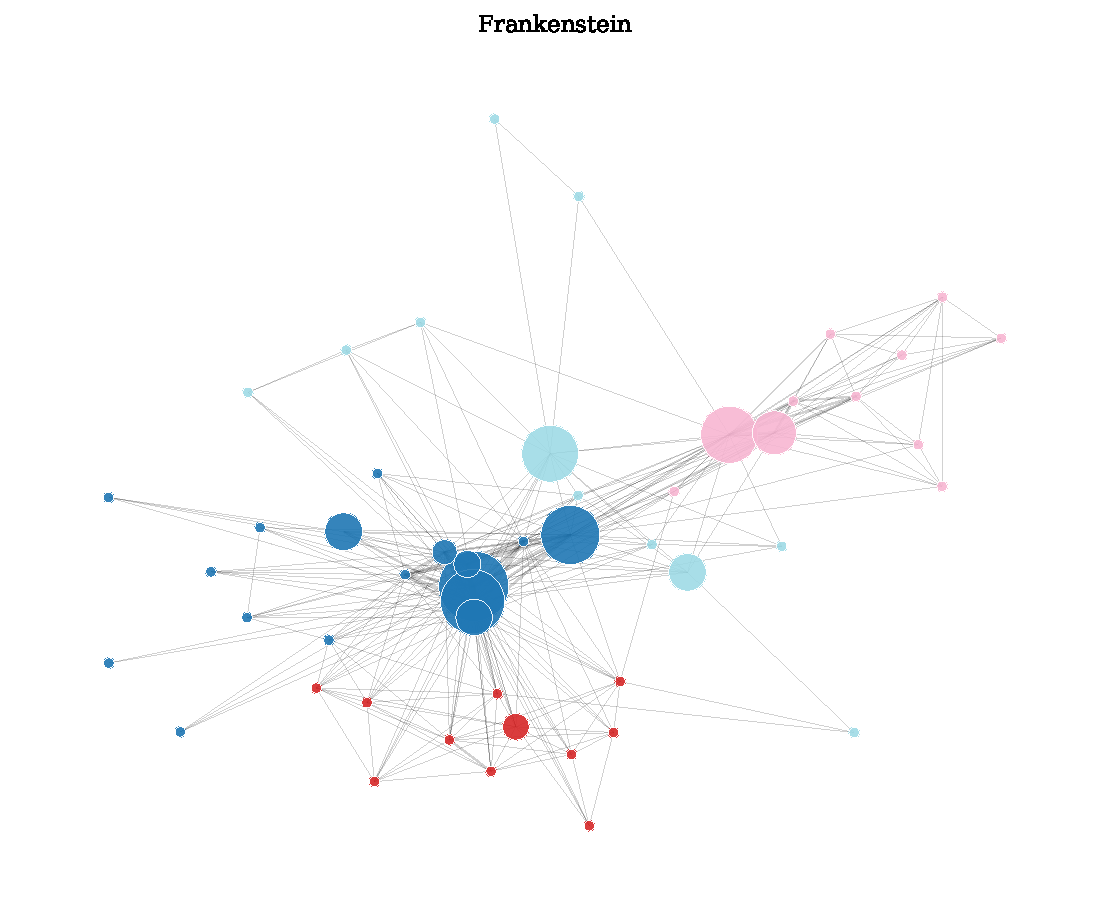
\includegraphics[width=0.74\textwidth]{figures/net_frankenstein.pdf}\caption{Character co-occurrence network of \emph{Frankenstein}. Node size is proportional to betweenness and colours denote communities (greedy modularity); the most central characters are named in the accompanying table.}\end{figure}

\begin{table}[H]\centering\small
\begin{tabular}{lrrrr}
\toprule
Character & $C_B$ & Degree & Closeness & Eigenvector \\
\midrule
Elizabeth & 0.550 & 36 & 9.66 & 0.507 \\
Clerval & 0.380 & 36 & 9.43 & 0.402 \\
God & 0.271 & 24 & 9.11 & 0.257 \\
Felix & 0.240 & 23 & 6.79 & 0.050 \\
Frankenstein (\#151) & 0.233 & 17 & 8.39 & 0.096 \\
Safie & 0.079 & 18 & 6.32 & 0.035 \\
Mr. Kirwin & 0.041 & 8 & 7.34 & 0.077 \\
Margaret & 0.040 & 11 & 5.96 & 0.039 \\
Victor & 0.035 & 26 & 9.03 & 0.352 \\
William & 0.009 & 26 & 8.96 & 0.366 \\
\bottomrule
\end{tabular}
\caption{Top-10 characters in \emph{Frankenstein} ranked by betweenness.}\end{table}
\clearpage

\subsection{A Tale of Two Cities (Dickens, 1859)}

\begin{figure}[H]\centering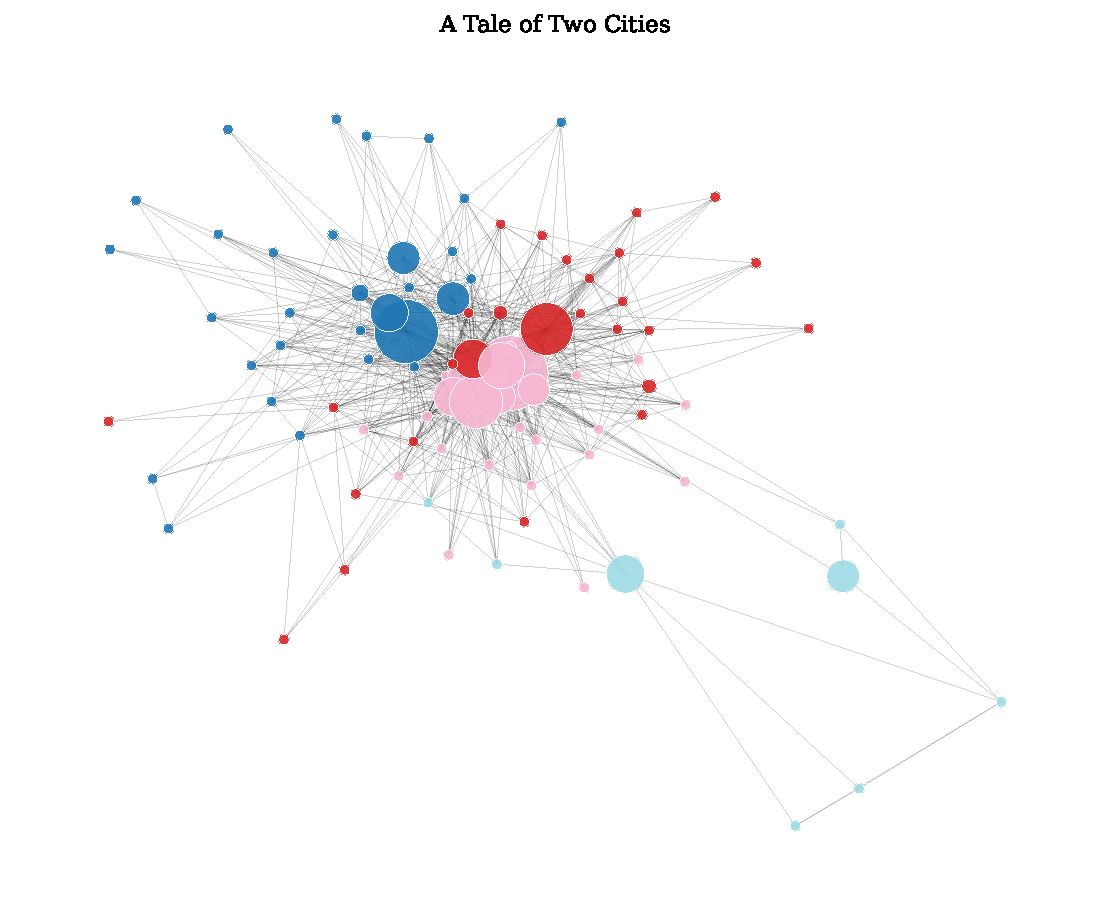
\includegraphics[width=0.74\textwidth]{figures/net_a-tale-of-two-cities.pdf}\caption{Character co-occurrence network of \emph{A Tale of Two Cities}. Node size is proportional to betweenness and colours denote communities (greedy modularity); the most central characters are named in the accompanying table.}\end{figure}

\begin{table}[H]\centering\small
\begin{tabular}{lrrrr}
\toprule
Character & $C_B$ & Degree & Closeness & Eigenvector \\
\midrule
Mr. Lorry & 0.695 & 60 & 15.11 & 0.468 \\
Madame Defarge & 0.382 & 48 & 14.45 & 0.215 \\
Darnay & 0.282 & 55 & 14.78 & 0.404 \\
Lucie & 0.179 & 47 & 14.60 & 0.356 \\
Mr. Cruncher & 0.171 & 46 & 13.62 & 0.126 \\
Miss Pross & 0.100 & 41 & 14.48 & 0.278 \\
Carton & 0.050 & 46 & 13.74 & 0.237 \\
Doctor Manette & 0.047 & 47 & 14.48 & 0.328 \\
Death & 0.044 & 11 & 5.43 & 0.007 \\
Saint Antoine & 0.043 & 36 & 12.96 & 0.062 \\
\bottomrule
\end{tabular}
\caption{Top-10 characters in \emph{A Tale of Two Cities} ranked by betweenness.}\end{table}
\clearpage

\subsection{Dracula (Stoker, 1897)}

\begin{figure}[H]\centering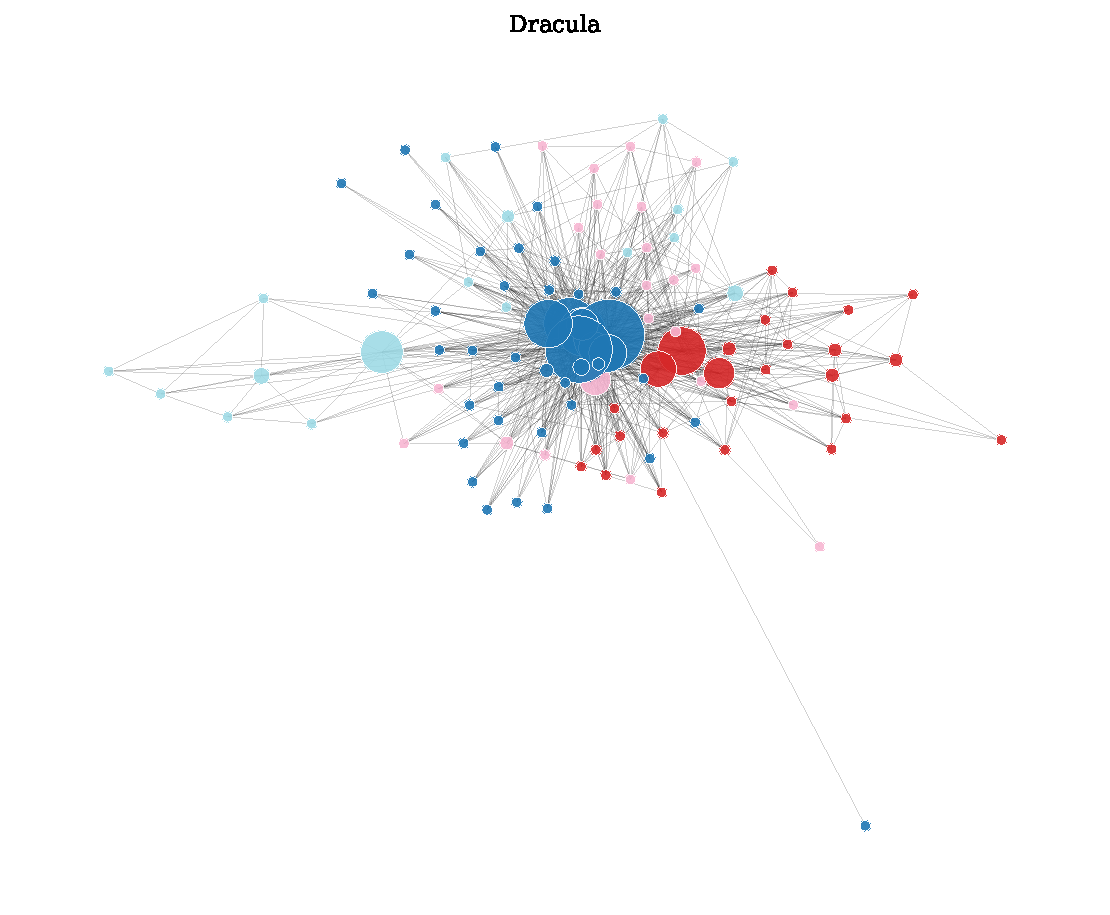
\includegraphics[width=0.74\textwidth]{figures/net_dracula.pdf}\caption{Character co-occurrence network of \emph{Dracula}. Node size is proportional to betweenness and colours denote communities (greedy modularity); the most central characters are named in the accompanying table.}\end{figure}

\begin{table}[H]\centering\small
\begin{tabular}{lrrrr}
\toprule
Character & $C_B$ & Degree & Closeness & Eigenvector \\
\midrule
Jonathan & 0.589 & 98 & 12.92 & 0.440 \\
Van Helsing (\#335) & 0.461 & 86 & 12.89 & 0.461 \\
Lucy & 0.162 & 76 & 12.78 & 0.361 \\
Renfield & 0.119 & 50 & 12.11 & 0.123 \\
Count Dracula & 0.118 & 46 & 11.47 & 0.047 \\
Dr. Seward & 0.116 & 88 & 12.77 & 0.347 \\
Lor & 0.069 & 21 & 6.97 & 0.007 \\
Lord Godalming & 0.042 & 63 & 12.60 & 0.247 \\
Galatz & 0.035 & 35 & 10.95 & 0.048 \\
Arthur & 0.019 & 69 & 12.63 & 0.300 \\
\bottomrule
\end{tabular}
\caption{Top-10 characters in \emph{Dracula} ranked by betweenness.}\end{table}
\clearpage

\subsection{Great Expectations (Dickens, 1861)}

\begin{figure}[H]\centering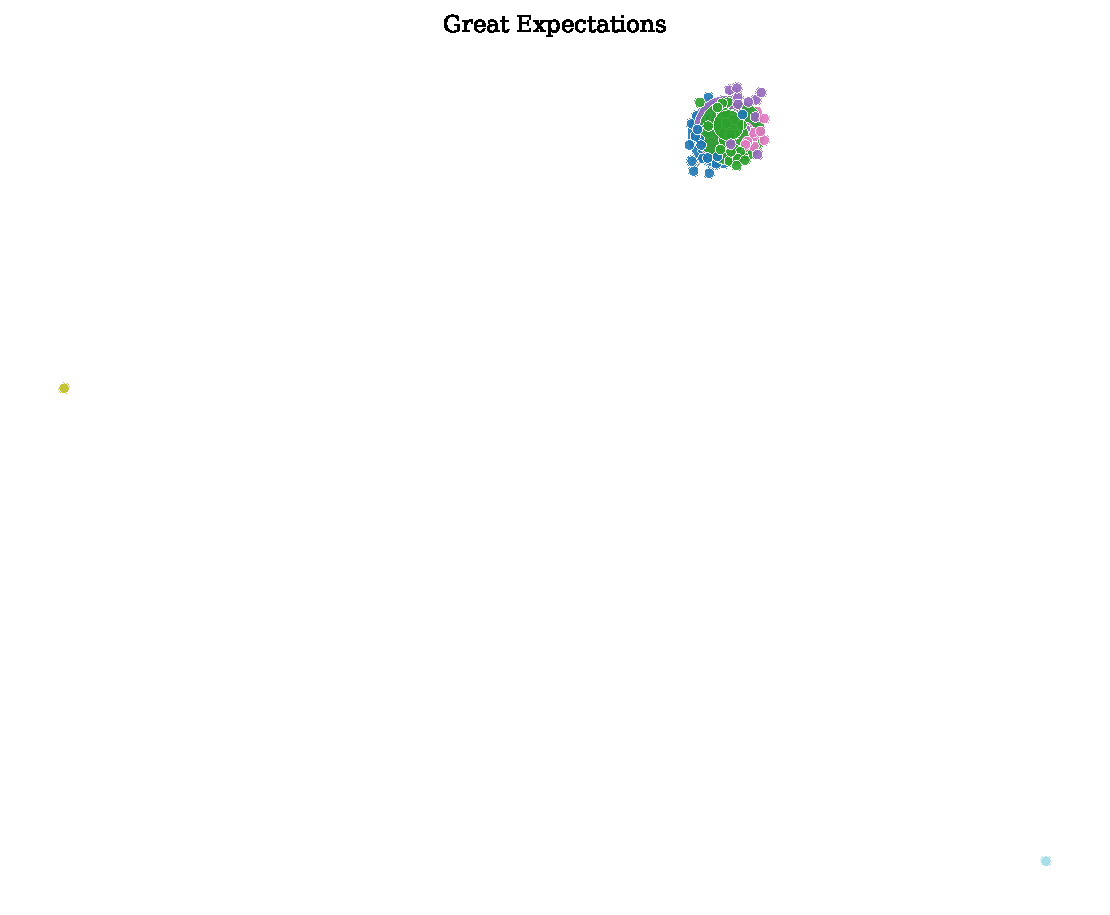
\includegraphics[width=0.74\textwidth]{figures/net_great-expectations.pdf}\caption{Character co-occurrence network of \emph{Great Expectations}. Node size is proportional to betweenness and colours denote communities (greedy modularity); the most central characters are named in the accompanying table.}\end{figure}

\begin{table}[H]\centering\small
\begin{tabular}{lrrrr}
\toprule
Character & $C_B$ & Degree & Closeness & Eigenvector \\
\midrule
Joe & 0.496 & 87 & 18.77 & 0.409 \\
Pip & 0.456 & 101 & 18.88 & 0.472 \\
Herbert & 0.449 & 84 & 18.49 & 0.258 \\
Miss Havisham & 0.228 & 74 & 18.70 & 0.427 \\
Wemmick & 0.139 & 59 & 18.21 & 0.191 \\
Mr. Jaggers & 0.098 & 63 & 18.20 & 0.239 \\
Estella & 0.066 & 70 & 18.21 & 0.325 \\
Mr. Pumblechook & 0.049 & 48 & 17.83 & 0.176 \\
Sarah Pocket & 0.032 & 28 & 16.40 & 0.076 \\
Mr. Pocket & 0.027 & 35 & 15.45 & 0.070 \\
\bottomrule
\end{tabular}
\caption{Top-10 characters in \emph{Great Expectations} ranked by betweenness.}\end{table}
\clearpage

\subsection{Huckleberry Finn (Twain, 1884)}

\begin{figure}[H]\centering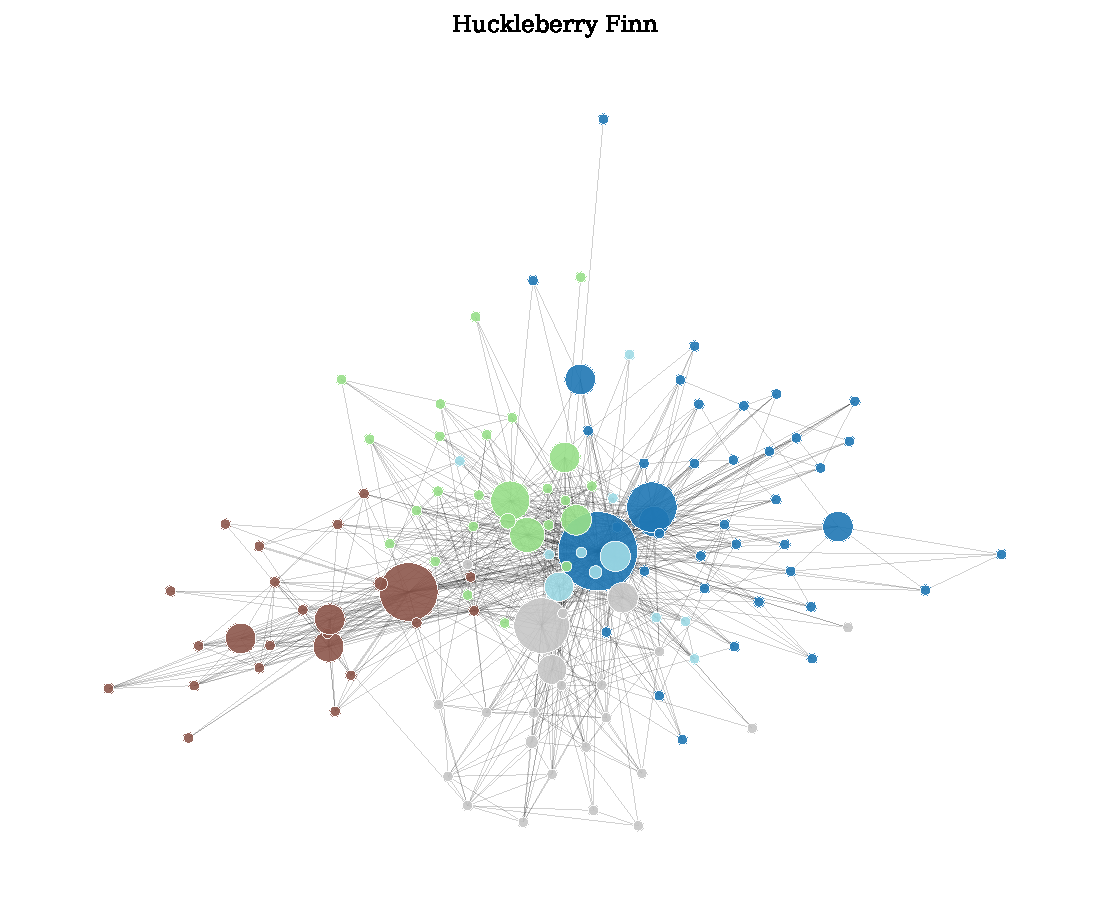
\includegraphics[width=0.74\textwidth]{figures/net_huckleberry-finn.pdf}\caption{Character co-occurrence network of \emph{Huckleberry Finn}. Node size is proportional to betweenness and colours denote communities (greedy modularity); the most central characters are named in the accompanying table.}\end{figure}

\begin{table}[H]\centering\small
\begin{tabular}{lrrrr}
\toprule
Character & $C_B$ & Degree & Closeness & Eigenvector \\
\midrule
Jim & 0.901 & 108 & 13.02 & 0.615 \\
Mary Jane & 0.263 & 49 & 10.57 & 0.088 \\
Buck & 0.211 & 46 & 11.07 & 0.109 \\
Aunt Sally & 0.140 & 44 & 12.43 & 0.358 \\
Bill & 0.048 & 35 & 9.58 & 0.075 \\
Pap & 0.029 & 42 & 11.52 & 0.161 \\
Peter & 0.017 & 26 & 8.92 & 0.023 \\
Harvey & 0.016 & 17 & 9.05 & 0.021 \\
Dey & 0.016 & 29 & 10.70 & 0.089 \\
Sherburn & 0.016 & 20 & 6.48 & 0.041 \\
\bottomrule
\end{tabular}
\caption{Top-10 characters in \emph{Huckleberry Finn} ranked by betweenness.}\end{table}
\clearpage

\subsection{The Adventures of Sherlock Holmes (Doyle, 1892)}

\begin{figure}[H]\centering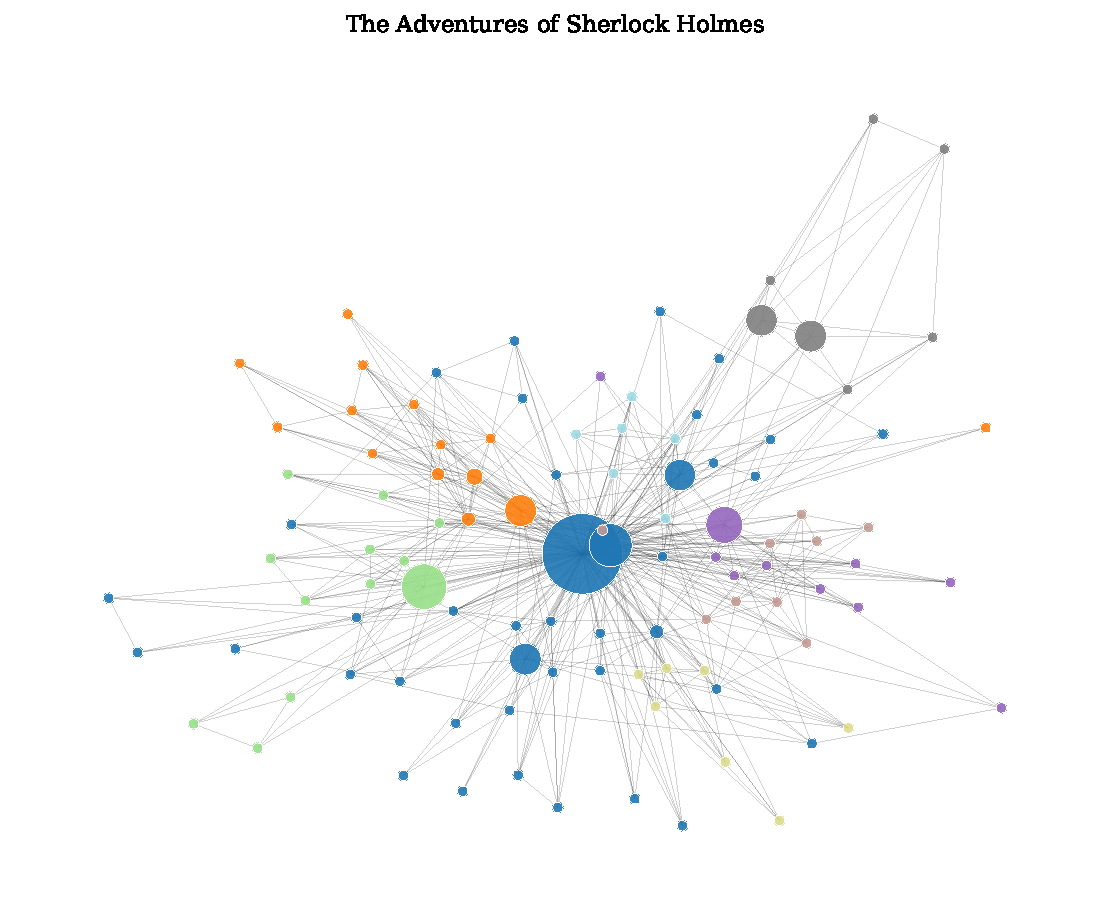
\includegraphics[width=0.74\textwidth]{figures/net_sherlock-holmes.pdf}\caption{Character co-occurrence network of \emph{The Adventures of Sherlock Holmes}. Node size is proportional to betweenness and colours denote communities (greedy modularity); the most central characters are named in the accompanying table.}\end{figure}

\begin{table}[H]\centering\small
\begin{tabular}{lrrrr}
\toprule
Character & $C_B$ & Degree & Closeness & Eigenvector \\
\midrule
Holmes & 0.971 & 102 & 18.97 & 0.655 \\
Lord St. Simon & 0.093 & 15 & 16.62 & 0.132 \\
Watson & 0.073 & 76 & 18.34 & 0.487 \\
Miss Hunter & 0.037 & 18 & 16.47 & 0.131 \\
Isa Whitney & 0.019 & 10 & 8.30 & 0.019 \\
Mr. Hatherley & 0.019 & 17 & 14.68 & 0.058 \\
Irene Adler & 0.019 & 12 & 15.62 & 0.081 \\
John Openshaw & 0.018 & 20 & 14.89 & 0.084 \\
Kate & 0.018 & 9 & 8.84 & 0.021 \\
young McCarthy & 0.001 & 16 & 16.43 & 0.134 \\
\bottomrule
\end{tabular}
\caption{Top-10 characters in \emph{The Adventures of Sherlock Holmes} ranked by betweenness.}\end{table}
\clearpage

\subsection{Emma (Austen, 1815)}

\begin{figure}[H]\centering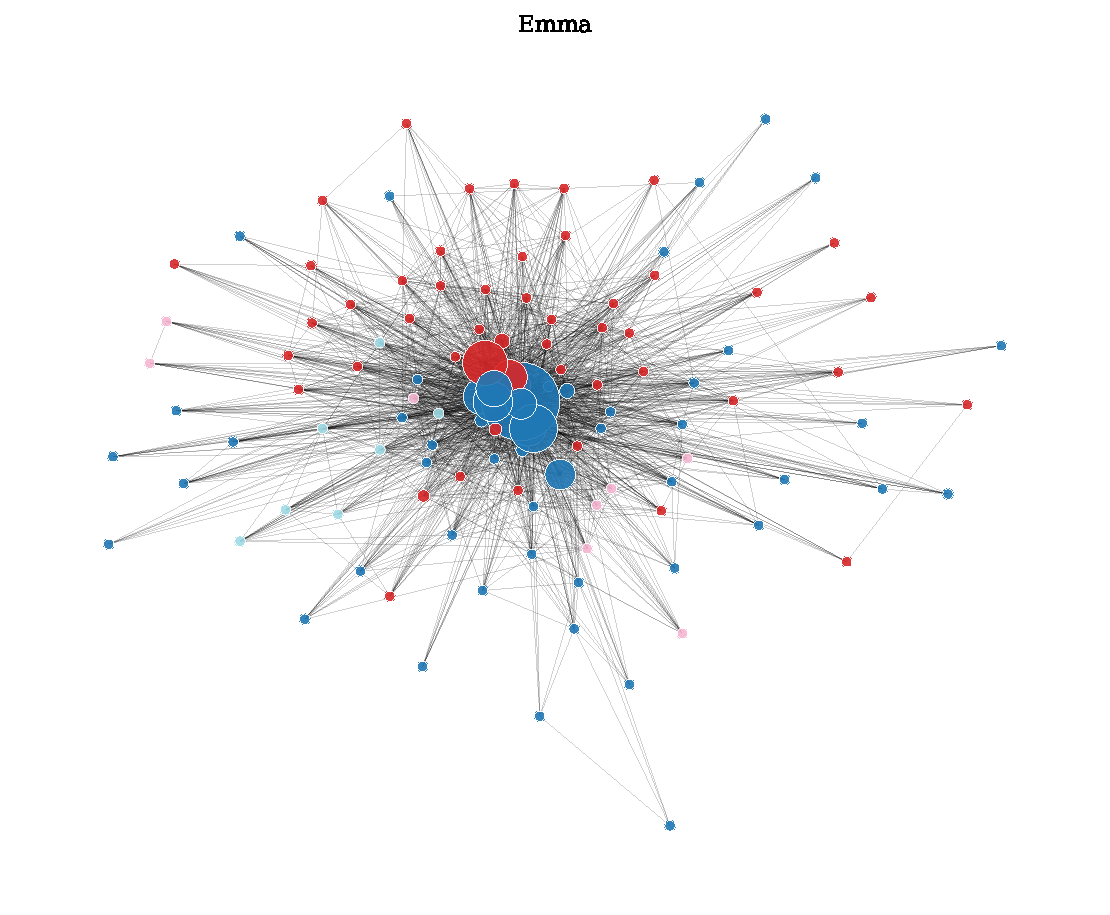
\includegraphics[width=0.74\textwidth]{figures/net_emma.pdf}\caption{Character co-occurrence network of \emph{Emma}. Node size is proportional to betweenness and colours denote communities (greedy modularity); the most central characters are named in the accompanying table.}\end{figure}

\begin{table}[H]\centering\small
\begin{tabular}{lrrrr}
\toprule
Character & $C_B$ & Degree & Closeness & Eigenvector \\
\midrule
Emma & 0.861 & 118 & 20.05 & 0.479 \\
Harriet & 0.116 & 103 & 19.78 & 0.307 \\
Mrs. Elton & 0.087 & 78 & 19.32 & 0.153 \\
Mrs. Weston & 0.051 & 95 & 19.71 & 0.299 \\
Mr. Knightley (\#281) & 0.034 & 100 & 19.76 & 0.320 \\
Mr. Weston & 0.034 & 88 & 19.54 & 0.236 \\
Mr. Elton & 0.033 & 92 & 19.55 & 0.212 \\
Miss Fairfax & 0.028 & 93 & 19.66 & 0.250 \\
Miss Woodhouse & 0.019 & 101 & 19.62 & 0.261 \\
Mr. Woodhouse & 0.017 & 103 & 19.50 & 0.220 \\
\bottomrule
\end{tabular}
\caption{Top-10 characters in \emph{Emma} ranked by betweenness.}\end{table}
\clearpage

\subsection{Jane Eyre (Brontë, 1847)}

\begin{figure}[H]\centering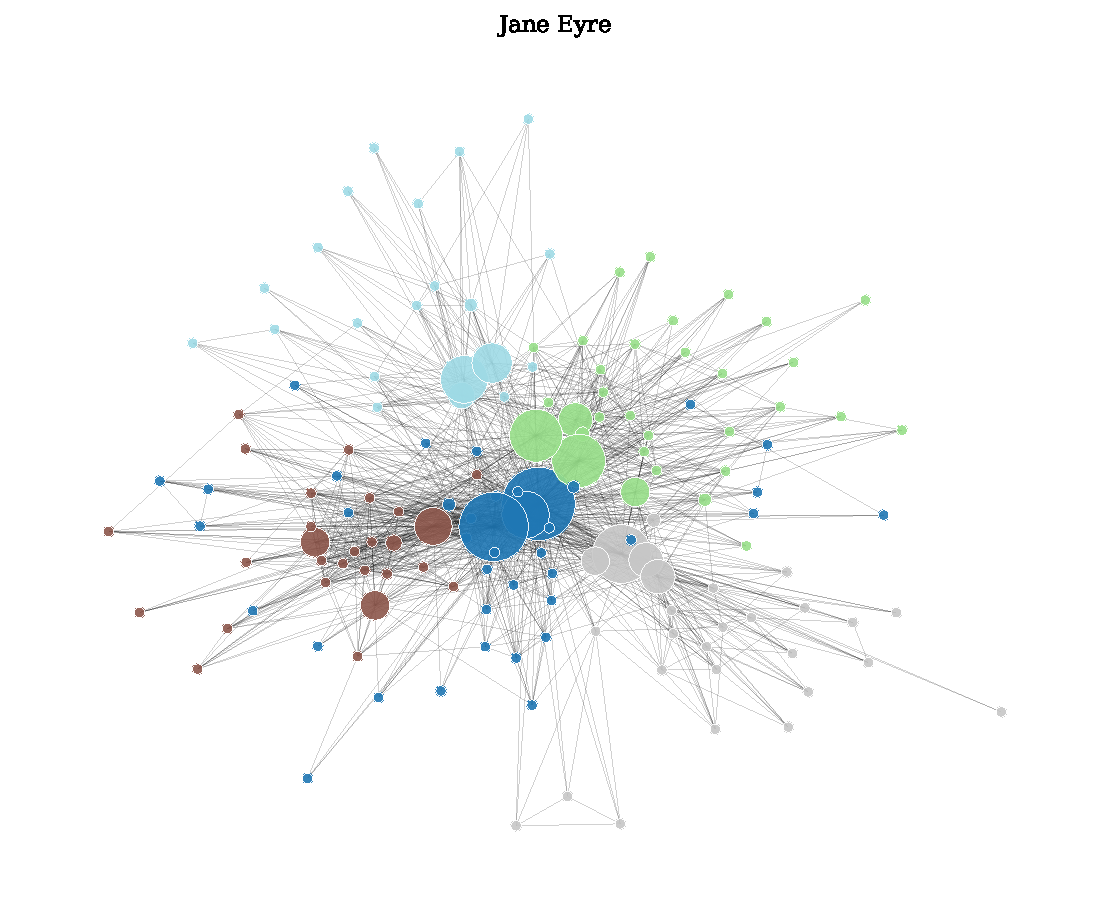
\includegraphics[width=0.74\textwidth]{figures/net_jane-eyre.pdf}\caption{Character co-occurrence network of \emph{Jane Eyre}. Node size is proportional to betweenness and colours denote communities (greedy modularity); the most central characters are named in the accompanying table.}\end{figure}

\begin{table}[H]\centering\small
\begin{tabular}{lrrrr}
\toprule
Character & $C_B$ & Degree & Closeness & Eigenvector \\
\midrule
Jane & 0.662 & 103 & 17.52 & 0.460 \\
Mr. Rochester & 0.523 & 101 & 17.42 & 0.498 \\
St. John & 0.265 & 66 & 16.81 & 0.252 \\
Bessie & 0.181 & 72 & 16.72 & 0.195 \\
Mrs. Reed & 0.171 & 65 & 16.66 & 0.139 \\
Miss Temple & 0.111 & 31 & 14.99 & 0.053 \\
Mrs. Fairfax & 0.107 & 113 & 17.30 & 0.453 \\
Helen & 0.054 & 26 & 14.85 & 0.039 \\
Miss Ingram & 0.040 & 50 & 16.24 & 0.131 \\
Mary & 0.027 & 40 & 15.99 & 0.125 \\
\bottomrule
\end{tabular}
\caption{Top-10 characters in \emph{Jane Eyre} ranked by betweenness.}\end{table}
\clearpage

\end{document}
